\subsubsection{Data in the blocks}
The pages allocated to a given object (table, index, etc) are managed through lists, which are stored as part of the segment header
\begin{figure}[h!]
    \begin{center}
        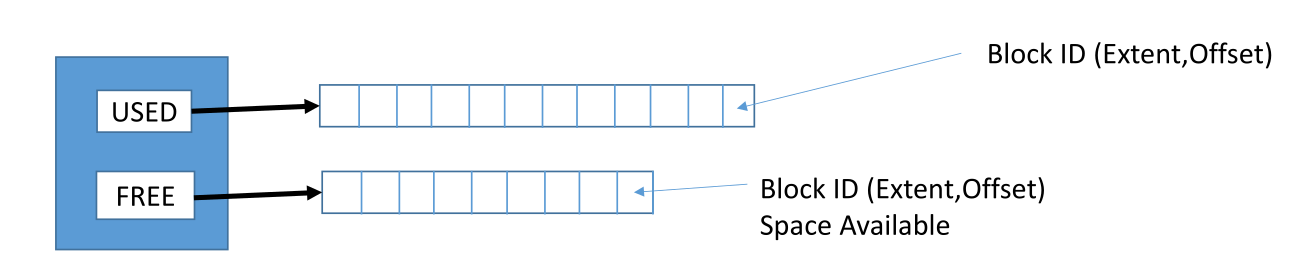
\includegraphics[width=0.9\columnwidth]{assets/db-system-page-lists.png}
    \end{center}
    \caption{Free/used lists in databases
        (Figure from Lecture 09, Slide 24)}
\end{figure}

These lists can become a bottleneck, especially for transactions that result in modifications.
There are some ways to improve the performance:
\begin{itemize}
    \item We can use several free lists, so concurrent transactions can find free space in parallel, rather than having conflicts all the time
    \item Make the traversal of the list faster (sorting, etc)
    \item Make sure that holes can be found efficiently (store the available space in each page in incremental steps)
\end{itemize}


\paragraph{Slotted Pages}
To find tuples within pages, slotted pages are used often.
In slotted pages, each page has a header containing checksum, version, transaction visibility, compression information, utilization, etc.

Then, each tuple gets an id (typically a block ID and an offset).

The page maintains a list of the ``slots'' (each slot is assigned to one tuple and thus the number of tuples in the pages is further constrained by the number of pages available).
The offsets, or sometimes pointers, are stored at the beginning of each tuple.

Advantages of slotted pages are:
\begin{itemize}
    \item storing tuples of different sizes (and variable length tuples)
    \item Each tuple gets a permanent tuple / record id, that does not change
    \item When data doesn't change, space is used efficiently
    \item When data \textit{does} change, we need to be careful
\end{itemize}

Considerations for when data \textit{does} change:
\begin{itemize}
    \item If a tuple is modified and becomes larger, the original space is used to store a pointer to the new location of the tuple
    \item If a tuple is deleted, we just remove the pointer
    \item If a tuple is modified and becomes smaller, leave the unnecessary space empty
    \item For insertion, we look for a page with enough free space and compact the page, if needed
\end{itemize}

The percentage free measure is used to avoid fragmentation caused by pages running out of space to accommodate updates for tuples that become larger.
Thus, some space is reserved for growing the tuples, rather than for inserting.

Without this measure, the block can constantly go from \texttt{FREE} to \texttt{USED} and back and forth.
